\documentclass[conference]{IEEEtran}

\usepackage{amsmath,amssymb}
\usepackage{booktabs}
\usepackage{graphicx}
\usepackage{url}

\title{Zero-UX-Loss Energy Optimization and Live EnergyTrace Analysis of an Autonomous MSP430FR5994 Roguelike}

\author{\IEEEauthorblockN{joaogpd}
\IEEEauthorblockA{\textit{mspgame Embedded Systems Project} \\
TI MSP430FR5994 LaunchPad Platform}}

\begin{document}

\maketitle

\begin{abstract}
Interactive embedded applications with high-speed asynchronous serial interfaces face a fundamental trade-off between deep low-power sleep modes and single-byte wake-up reliability. We present a low-level power audit, Tier~1 Zero-UX-Loss firmware optimization, silicon wake-up investigation, and live Texas Instruments (TI) Code Composer Studio (CCS) EnergyTrace evaluation of \texttt{mspgame}, an 80$\times$24 ANSI/VT100 roguelike with on-chip Q7 autonomous AI policies running on the TI MSP430FR5994 LaunchPad (\texttt{115200}~baud 8N1 UART). Empirical hardware testing proves that \texttt{PMM\_LPM3} with \texttt{SMCLKREQEN} drops single-byte cold-idle wakeups (\texttt{IDLE\_1BYTE}=0 vs.\ \texttt{IDLE\_2BYTE}=1,043~bytes) because \texttt{LPM3} and FRAM wake-up latencies ($6.85$--$9.91~\mu\text{s} + 6$--$10~\mu\text{s}$) exceed the $4.34~\mu\text{s}$ start-bit midpoint at \texttt{115200}~baud and conflict with silicon erratum \texttt{PMM31}. By scaling the DCO uniformly to 4~MHz, sleeping in \texttt{PMM\_LPM1} when UART TX is idle (\texttt{PMM\_LPM0} during TX shifts), dynamically gating \texttt{TIMER\_A1} to 0~Hz during connected idle and manual play, pulsing Red \texttt{LED1} for 25~ms via \texttt{TIMER\_A2} with minimal Row~1/2 Low-HP redraws, and fixing Port~9/clock/PMM driver leakage, the firmware passes 8/8 live \texttt{COM4} reliability checks (10/10 cold-idle wakeups) with 0~errors and 0~warnings. Across 30.00~s EnergyTrace captures ($V_{\text{mean}}=3.289$--$3.290\text{~V}$), true energy-derived current $I_{\text{ev}}$ drops by 64.05\% ($2.78\times$) in Idle ($192.78\rightarrow 69.29~\mu\text{A}$), 43.67\% ($1.78\times$) in Active Play ($245.19\rightarrow 138.11~\mu\text{A}$), 44.61\%--52.16\% ($1.81\times$--$2.09\times$) against active 8~MHz Baseline AI ($447.64\rightarrow 247.93~\mu\text{A}$ Heuristic~A; $214.16~\mu\text{A}$ Tiny-MLP~B), and 87.54\% ($8.02\times$) in Low-HP Alert ($1,953.00\rightarrow 243.38~\mu\text{A}$), extending CR2032 runtime up to 120.63~days and LaunchPad supercapacitor \texttt{C1} (0.22~F) runtime up to 61.52~min.
\end{abstract}

\begin{IEEEkeywords}
MSP430FR5994, EnergyTrace, Low-Power Embedded Systems, LPM1, UART Wake-up Latency, Silicon Errata, FRAM.
\end{IEEEkeywords}

\section{Introduction}
Ultra-low-power 16-bit Ferroelectric RAM (FRAM) microcontrollers such as the Texas Instruments MSP430FR5994 offer sub-microampere standby currents, yet real-world interactive peripherals impose strict timing and errata boundaries on achievable sleep depth. In \texttt{mspgame}~\cite{mspgame_ga}, a procedural 48$\times$22 roguelike rendered over an 80$\times$24 ANSI/VT100 backchannel UART at \texttt{115200}~baud (8N1) with autonomous on-chip Q7 AI modes (22~B Heuristic~A and 587~B Tiny-MLP~B), the Baseline firmware (\texttt{5cf488d}) operated at 8~MHz DCO, slept solely in \texttt{LPM0}, ran a continuous 2~Hz \texttt{TIMER\_A1} wakeup, and toggled Red \texttt{LED1} at 50\% duty cycle during critical Low-HP alerts.

This paper presents a systematic register-level audit and Tier~1 \emph{Zero-UX-Loss} energy optimization campaign that preserves \texttt{115200}~baud responsiveness, full 80$\times$24 ANSI color fidelity, and 500~ms AI Demo cadence. Our contributions are:
\begin{enumerate}
    \item \textbf{Silicon Wake-Up \& Errata Resolution:} Quantitative physics and live \texttt{COM4} proof showing why \texttt{LPM3 + SMCLKREQEN} drops single-byte \texttt{115200}~baud commands, and how \texttt{PMM\_LPM1 @ 4~MHz} achieves 10/10 cold-idle RX reliability with zero \texttt{PMM31}/\texttt{PMM32} errata~\cite{ti_ds,ti_errata}.
    \item \textbf{Tier~1 Driver \& Firmware Fixes:} Dynamic 0~Hz \texttt{TIMER\_A1} gating, 25~ms \texttt{TIMER\_A2} \texttt{LED1} one-shot pulses with minimal Row~1/2 redraws, \texttt{CSCTL4}/\texttt{CSCTL6} oscillator gating, Port~9 low-power initialization, and \texttt{PMM32}-safe FRAM power control~\cite{ti_ug}.
    \item \textbf{EnergyTrace Validation \& Filter Artifact Analysis:} Reproducible 30~s Baseline vs.\ Optimized EnergyTrace benchmarks across five profiles, sub-second 5~ms \texttt{Energy (uJ)} slope decomposition explaining TI's \texttt{EnergyTraceRunningAverageFilter} hold tail, datasheet reconciliation, and CR2032 / \texttt{C1} supercapacitor lifetime projections.
\end{enumerate}

\section{Low-Level Power Audit \& Tier 1 Optimizations}

Auditing \texttt{main.c}, \texttt{drivers/board/board.c}, \texttt{drivers/msp430/} (\texttt{cs}, \texttt{pmm}, \texttt{uart}, \texttt{gpio}, \texttt{timer}), and \texttt{app/dungeon\_game.c} against the MSP430FR5994 datasheet~\cite{ti_ds}, Family User's Guide~\cite{ti_ug}, and Silicon Errata~\cite{ti_errata} exposed seven defects in the \texttt{5cf488d} Baseline:
\begin{itemize}
    \item \textbf{Clock Scaling \& Sleep Mode (\texttt{main.c}):} Baseline ran \texttt{CS\_DCO\_8MHZ} and \texttt{LPM0} ($190~\mu\text{A}$ typ). Optimized firmware configures \texttt{CS\_DCO\_4MHZ} ($MCLK = SMCLK = 4\text{~MHz}$), flushes UART TX in \texttt{PMM\_LPM0}, and enters \texttt{PMM\_LPM1} whenever \texttt{uart\_tx\_idle(UART\_A0)} is true.
    \item \textbf{Oscillator \& Clock-Request Gating (\texttt{cs.c}, \texttt{cs.h}):} \texttt{CS\_CONFIG\_DEFAULT} enables \texttt{lfxt\_low\_drive = true} (\texttt{LFXTDRIVE\_0} for 32.768~kHz \texttt{Q1}); \texttt{cs\_init()} sets \texttt{CSCTL4 |= HFXTOFF}, enables \texttt{VLOOFF} once LFXT locks, sets \texttt{CSCTL6 = ACLKREQEN | MCLKREQEN | SMCLKREQEN | MODCLKREQEN}, and retains the \texttt{CS12} $\ge /4$ divider guard during DCO updates.
    \item \textbf{Dynamic \texttt{TIMER\_A1} Gating (\texttt{dungeon\_game.c}):} Baseline woke CPU and FRAM at 2~Hz unconditionally. \texttt{need\_probe\_timer()} and \texttt{sync\_probe\_timer()} now enable \texttt{TIMER\_A1} only when \texttt{!s\_terminal\_connected} (DSR probe), \texttt{s\_ai\_demo} is actively stepping, or \texttt{is\_low\_hp()} is active---yielding 0~Hz timer wakeups during connected idle and normal play while mixing \texttt{TA1R}/\texttt{TA0R} into \texttt{s\_entropy} before stopping.
    \item \textbf{Low-Duty \texttt{LED1} \& Minimal Redraw (\texttt{dungeon\_game.c}):} Baseline toggled Red \texttt{LED1} (\texttt{P1.0}, $\sim$3.26--3.35~mA across R24 $= 470~\Omega$~\cite{ti_lp}) at 50\% duty and resent a $\sim$430~B sidebar every 500~ms. Optimized firmware triggers a 25~ms \texttt{TIMER\_A2} one-shot pulse (\texttt{on\_led\_off\_timer()} returns \texttt{false} to remain in \texttt{LPM1}) and sets \texttt{s\_pulse\_only\_dirty} to emit a $\sim$138~B Row~1/2 ANSI update (\texttt{BEL} remains every 2.0~s).
    \item \textbf{PMM, UART, \& GPIO Driver Fixes (\texttt{pmm.c}, \texttt{uart.c}, \texttt{gpio.c}):} \texttt{pmm\_lpm\_from\_ram()} wraps \texttt{FRCTL0\_H} unlock and \texttt{FRPWR=0} with \texttt{\_\_disable\_interrupt()} inside \texttt{.TI.ramfunc} for \texttt{PMM32} compliance while keeping \texttt{SVSHE=1}. \texttt{uart.c} records \texttt{s\_u[id].clk} so \texttt{uart\_write\_all()} and \texttt{uart\_flush()} sleep in \texttt{PMM\_LPM0} (never \texttt{LPM3}) on \texttt{SMCLK}, eliminates \texttt{\%} ring-buffer modulo arithmetic, and polls \texttt{UCBUSY} (\texttt{USCI42}-safe). \texttt{gpio\_init\_all\_low\_power()} adds \texttt{GPIO\_PORT\_9} (\texttt{P9}) so all ports (\texttt{P1}--\texttt{P9}, \texttt{PJ}) initialize output-low before \texttt{pmm\_unlock\_io()}.
\end{itemize}

Compiled with TI CCS 12.5 \texttt{cl430 v21.6.1.LTS} (\texttt{--advice:power=all --advice:hw\_config=all}) with 0~errors, 0~warnings, and 0~new ULP remarks, \texttt{Debug/mspgame.map} reports 2,401/4,096~B \texttt{RAM} (58.62\%, 0~B heap), 0/4,096~B \texttt{LEARAM+LEASTACK}, 15,904/49,024~B lower \texttt{FRAM} (32.44\%), and 30,918/212,984~B upper \texttt{FRAM2} (14.52\%)—46,822/262,008~B total \texttt{FRAM+FRAM2} (17.87\%; 46,854~B including 32~B vectors/signatures).

\section{Silicon \texttt{LPM3} vs.\ \texttt{PMM\_LPM1 @ 4 MHz} Investigation}

Although \texttt{CSCTL6.SMCLKREQEN} allows \texttt{eUSCI\_A0} to request \texttt{SMCLK} in \texttt{LPM3}, testing the initial \texttt{PMM\_LPM3} build on physical hardware (\texttt{COM4 @ 115200}~baud 8N1) failed \texttt{tools/power\_bench.py --verify-uart}. After \texttt{MSP430\_Reset(0x0A, 1, 1)} and \texttt{0x0C} (\texttt{Ctrl+L}) transitioned the target into connected \texttt{LPM3} idle (\texttt{0~Hz} \texttt{TIMER\_A1}, \texttt{FRPWR=0}), sending a single byte \texttt{b"\textbackslash x0c"} produced \texttt{IDLE\_1BYTE = 0}~bytes, whereas sending two back-to-back bytes \texttt{b"\textbackslash x0c\textbackslash x0c"} yielded \texttt{IDLE\_2BYTE = 1,043}~bytes (exactly one redraw: byte~1 woke the DCO/FRAM with \texttt{UCRXERR} and was discarded by \texttt{on\_uart\_rx()}; byte~2 succeeded).

At \texttt{115200}~baud (8N1), one bit period is $8.68~\mu\text{s}$ and the start-bit midpoint is \textbf{$4.34~\mu\text{s}$} after the falling RX edge. Per \texttt{SLASE54}~\cite{ti_ds}, \texttt{LPM3} wake-up takes $t_{\text{WAKE-UP}} = 6.6~\mu\text{s} + 2/f_{\text{DCO}}$ ($6.85~\mu\text{s}$ typ, $9.91~\mu\text{s}$ max) plus $6$--$10~\mu\text{s}$ FRAM power-up from \texttt{FRPWR=0}. Even \texttt{PMM\_LPM2} ($6~\mu\text{s}$ typ) pushes sampling to $10.34~\mu\text{s} > 8.68~\mu\text{s}$, failing any key with $\text{LSB}=1$ (\texttt{`?'}, \texttt{`m'}, \texttt{`c'}). Moreover, erratum \texttt{PMM31}~\cite{ti_errata} restricts asynchronous \texttt{SMCLK} UART requests to \texttt{LPM0} or \texttt{LPM1}.

Switching to uniform \textbf{4~MHz \texttt{PMM\_LPM1}} (\texttt{SCG0=1, SCG1=0, FRPWR=1}) resolves both constraints:
\begin{enumerate}
    \item \textbf{Baud Margin:} \texttt{uart.c} (\texttt{SLAU367P} Table~30-4) sets \texttt{UCOS16=1, BRW=2, UCBRF=2, UCBRS=0xBB} ($N=34.7222$), giving $1.84\%$ max RX error and $2.24\%$ max TX error ($+0.08\%$ avg), well within $\pm 4.5\%$ UART tolerance (unlike 1.00~MHz at $16.88\%$ or 2.67~MHz at $5.04\%$).
    \item \textbf{Instant RX + Errata Exemption:} \texttt{LPM1} is exempt from \texttt{PMM31}/\texttt{PMM32} and keeps 4~MHz \texttt{SMCLK} active so \texttt{eUSCI\_A0} receives the full $86.8~\mu\text{s}$ frame before \texttt{UCRXIFG} wakes the CPU ($6~\mu\text{s} \ll 86.8~\mu\text{s}$).
    \item \textbf{Live Silicon Gate:} \texttt{power\_bench.py --port COM4 --verify-uart} passed \textbf{8/8 checks} on the first attempt, including 10/10 cold-idle ($1.5$--$2.7$~s) single-byte wakeups, 4/4 CSI arrows, 5/5 rapid bursts, 5,890 ANSI SGR sequences (0 errors), 0.499~s Heuristic / 0.496~s Tiny-MLP AI cadences, and 2 Low-HP \texttt{BEL} chimes over 5.8~s.
\end{enumerate}

\section{EnergyTrace Methodology \& Experimental Results}

\subsection{Measurement Protocol \& Filter Hold Artifact}
All captures followed \url{docs/power/CAPTURE_PROTOCOL.md}: LaunchPad powered over direct USB via eZ-FET \texttt{J101} (\texttt{3V3}, \texttt{TXD}, \texttt{RXD}, \texttt{SBWTDIO}, \texttt{SBWTCK} fitted), \texttt{J8=OFF} (isolating \texttt{C1}), empty microSD slot, \textbf{EnergyTrace (energy-only)} mode (\texttt{has\_dsr=false}), and \textbf{Free Run} execution for 30.00~s ($\sim$113k--115k samples, median $\Delta t=0.210\text{~ms}$). Baseline traces were exported from CCS 12.5 GUI; Optimized traces were captured in \texttt{continuous} mode via \url{tools/energytrace_capture.py} (\texttt{MSP430.dll}).

Because EnergyTrace derives current from DC-DC capacitor recharge pulses smoothed by TI's \texttt{EnergyTraceRunningAverageFilter}, sharp transitions from active TX ($\sim$640~$\mu\text{A}$) or \texttt{LED1} ($\sim$3.8~mA) down to 66~$\mu\text{A}$ \texttt{LPM1} leave sparse recharge intervals ($\sim$5~ms), causing \texttt{Current (nA)} ($I_{\text{tw}}$) to latch high for 100--175~ms ($V$--$I$ Diff up to 275.35\%). By contrast, the hardware \texttt{Energy (uJ)} accumulator gives the exact mean current $I_{\text{ev}} = E_{\text{tot}} / (T \cdot V_{\text{mean}})$. Sub-second 5~ms slope bins ($\Delta E / (\Delta t \cdot V_{\text{mean}})$) on \texttt{optimized\_low\_hp.csv} verify that energy accumulation drops to $5.42~\mu\text{J}$ ($65.9~\mu\text{A}$) immediately in $[0.175, 0.200\text{~s})$ right after the $[0.145, 0.170\text{~s})$ \texttt{LED1} pulse, with $<0.3\%$ per-second variance ($0.7980$--$0.8042\text{~mJ/s}$).

\begin{table*}[t]
\centering
\caption{Complete 30.00-Second CCS EnergyTrace Comparison: Baseline (\texttt{5cf488d}) vs.\ Optimized (\texttt{PMM\_LPM1 @ 4 MHz})}
\label{tab:summary}
\scriptsize
\setlength{\tabcolsep}{2.4pt}
\begin{tabular}{@{}llrrrrrrrrrrrl@{}}
\toprule
Profile & Variant & $N$ & $E_{\text{tot}}$ & $P_{\text{mean}}$ & $V_{\text{mean}}$ & $I_{\text{ev}}$ & $I_{\text{tw}}$ & $I_{p50}$ & $I_{p95}$ & $I_{\max}$ & $V$--$I$ & CR2032 / C1 & $\Delta P_{\text{mean}}$ \\
 & & & (mJ) & ($\mu$W) & (V) & ($\mu$A) & ($\mu$A) & ($\mu$A) & ($\mu$A) & ($\mu$A) & Diff (\%) & (d) / (min) & (vs.\ Base) \\
\midrule
Idle (Conn.) & Baseline & 115,246 & 19.023 & 634.11 & 3.289 & 192.78 & 192.20 & 189.9 & 193.4 & 827.2 & 0.30 & 43.37 / 22.12 & --- \\
Idle (Conn.) & Optimized & 115,484 & 6.839 & 227.96 & 3.290 & 69.29 & 68.66 & 69.2 & 69.6 & 69.9 & 0.90 & 120.63 / 61.52 & \textbf{-64.05\% (2.78$\times$)} \\
Active Play & Baseline & 114,782 & 24.195 & 806.50 & 3.289 & 245.19 & 261.84 & 190.0 & 744.2 & 1,219.4 & 6.79 & 34.10 / 17.39 & --- \\
Active Play & Optimized & 114,814 & 13.630 & 454.33 & 3.290 & 138.11 & 197.06 & 66.6 & 641.6 & 650.2 & 42.67 & 60.53 / 30.87 & \textbf{-43.67\% (1.78$\times$)} \\
AI: Heuristic A & Baseline* & 115,260 & 19.041 & 634.70 & 3.289 & 192.96 & 192.34 & 190.0 & 193.5 & 836.8 & 0.32 & 43.33 / 22.10 & --- \\
AI: Heuristic A & Optimized & 114,099 & 24.467 & 815.58 & 3.289 & 247.93 & 368.96 & 343.2 & 642.4 & 669.4 & 48.80 & 33.72 / 17.20 & +28.50\%* (\textbf{-44.61\%} act.) \\
AI: Tiny-MLP B & Baseline** & 114,923 & 22.527 & 750.89 & 3.289 & 228.28 & 232.36 & 190.2 & 525.6 & 1,218.7 & 1.79 & 36.62 / 18.68 & --- \\
AI: Tiny-MLP B & Optimized & 114,346 & 21.135 & 704.51 & 3.290 & 214.16 & 327.57 & 192.4 & 650.4 & 672.1 & 52.95 & 39.03 / 19.91 & -6.18\%** (\textbf{-52.16\%} act.) \\
Low-HP Alert & Baseline & 113,401 & 192.720 & 6,423.91 & 3.289 & 1,953.00 & 1,993.20 & 3,345.2 & 4,096.1 & 4,349.1 & 2.05 & 4.28 / 2.18 & --- \\
Low-HP Alert & Optimized & 115,109 & 24.020 & 800.69 & 3.290 & 243.38 & 913.57 & 100.5 & 3,260.0 & 3,864.7 & 275.35 & 34.35 / 17.52 & \textbf{-87.54\% (8.02$\times$)} \\
\bottomrule
\multicolumn{14}{@{}p{\textwidth}@{}}{\scriptsize * \texttt{baseline\_ai\_heuristic.csv} sat idle at $191.05$--$191.90~\mu\text{A}$ for $0$--$28.90\text{~s}$. ** \texttt{baseline\_ai\_mlp.csv} ran active AI in $[0,3\text{~s}]$ ($1,472.50~\mu\text{W}$, $447.64~\mu\text{A}$), then idled $4$--$28\text{~s}$.}
\end{tabular}
\end{table*}

\begin{figure}[t]
\centering
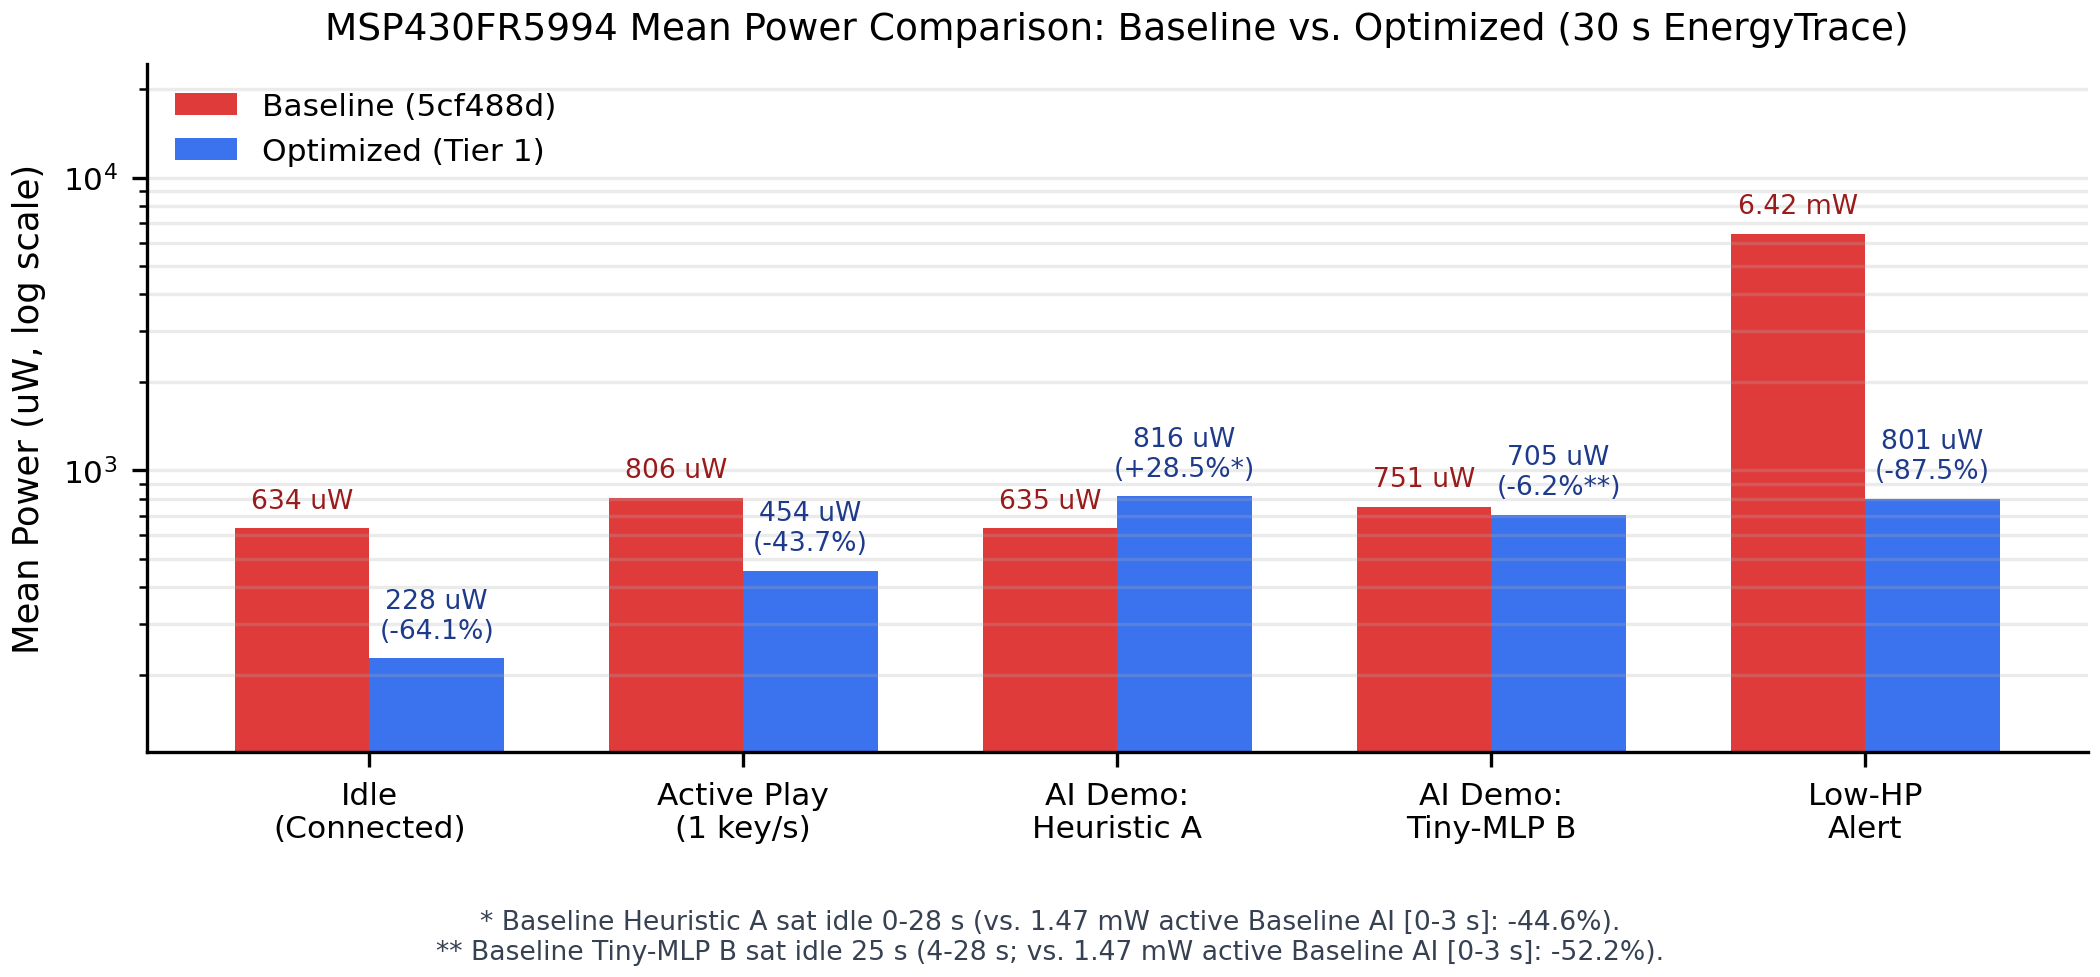
\includegraphics[width=\columnwidth]{figures/power_comparison.png}
\caption{Mean power across all five 30.00~s EnergyTrace profiles comparing Baseline (\texttt{5cf488d}) and Optimized Tier~1 (\texttt{PMM\_LPM1 @ 4~MHz}) firmware.}
\label{fig:power_comp}
\end{figure}

\begin{figure}[t]
\centering
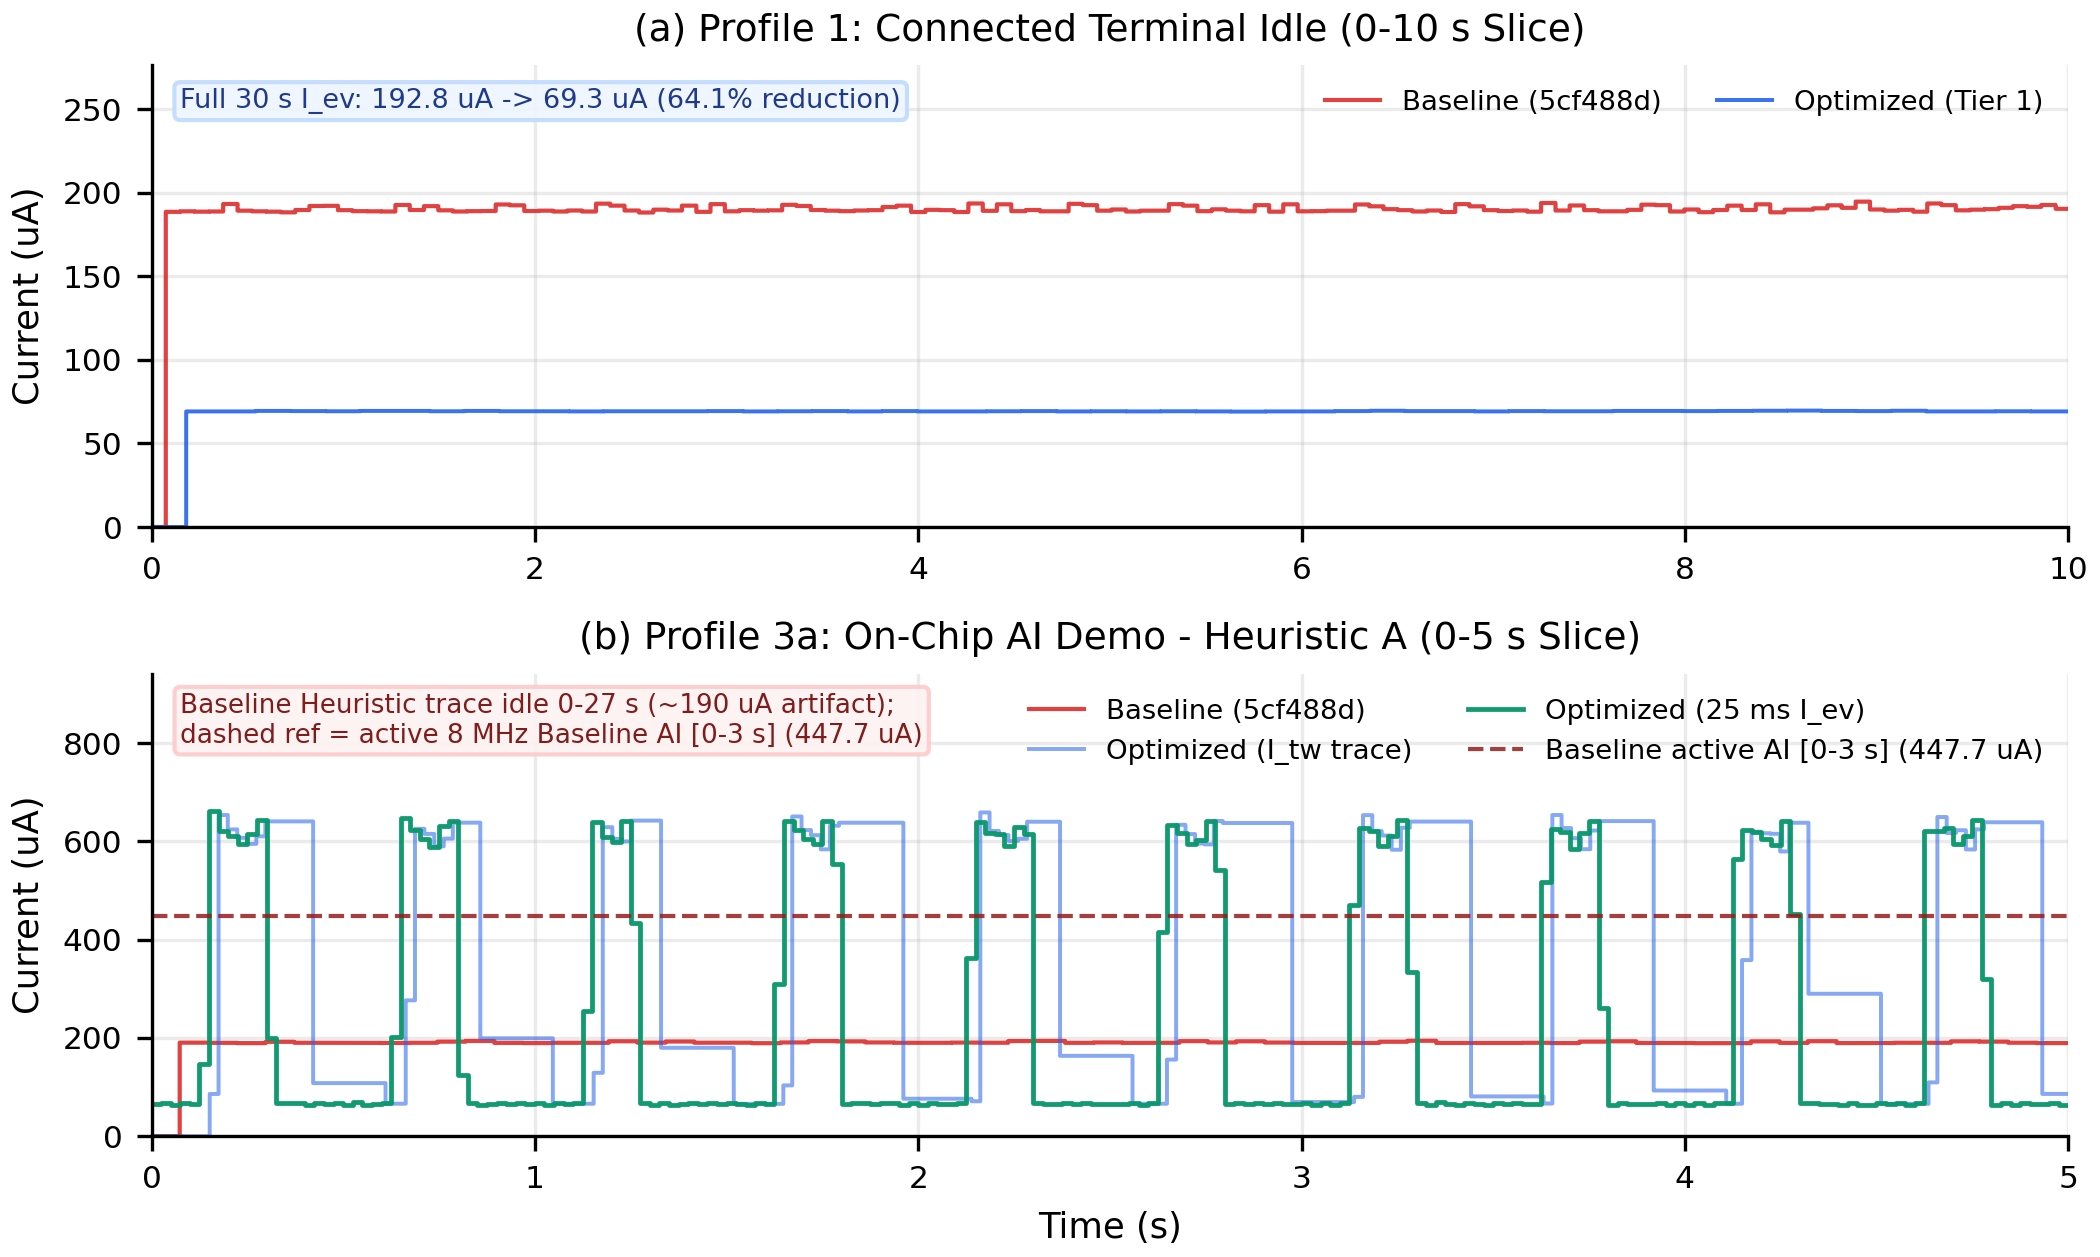
\includegraphics[width=\columnwidth]{figures/waveforms_idle_ai.png}
\caption{Measured current waveforms for (a) Connected Idle ($192.8\rightarrow 69.3~\mu\text{A}$) and (b) On-Chip AI Demo Heuristic~A showing 25~ms $I_{\text{ev}}$ vs.\ $I_{\text{tw}}$ filter hold.}
\label{fig:wave_idle_ai}
\end{figure}

\subsection{Quantitative Results \& Sub-Second Budgets}
Table~\ref{tab:summary} and Figs.~\ref{fig:power_comp}--\ref{fig:wave_low_hp} summarize all 10 captures:
\begin{itemize}
    \item \textbf{Idle \& Active Play:} Connected Idle drops 64.05\% ($634.11\rightarrow 227.96~\mu\text{W}$) with $I_{\max}=69.9~\mu\text{A}$ (zero timer wakeups). Active Play drops 43.67\% ($806.50\rightarrow 454.33~\mu\text{W}$) because inter-keystroke sleep drops from $191.07~\mu\text{A}$ to $66.40~\mu\text{A}$.
    \item \textbf{AI Demo \& Active Reference:} While \texttt{baseline\_ai\_heuristic.csv} sat idle for $0$--$28.90\text{~s}$, \texttt{baseline\_ai\_mlp.csv} executed genuine 8~MHz active AI during $[0.0, 3.0\text{~s}]$ ($\Delta E = 4.4172\text{~mJ}$, $P = 1,472.50~\mu\text{W}$, $I_{\text{ev}} = 447.64~\mu\text{A}$; $1,497.40~\mu\text{W}$ / $455.22~\mu\text{A}$ over $[0.0, 4.0\text{~s}]$). Against this active reference, continuous 60-tick \texttt{optimized\_ai\_heuristic} ($815.58~\mu\text{W}$) saves \textbf{44.61\%} ($1.81\times$) and \texttt{optimized\_ai\_mlp} ($704.51~\mu\text{W}$) saves \textbf{52.16\%} ($2.09\times$). Heuristic~A uses slightly more energy than Tiny-MLP~B because UART wire time ($86.8~\mu\text{s/B}$ in \texttt{LPM0}) dominates ($165\text{~ms}$ vs.\ $130\text{~ms}$ median active TX per tick) and Heuristic~A incurred two 320~ms / $656~\mu\text{J}$ death-restart full redraws at $t=16.58\text{~s}$ and $27.02\text{~s}$.
    \item \textbf{Low-HP Budget:} Replacing 50\% \texttt{LED1} + 430~B sidebar redraws ($6,204.1~\mu\text{J/cycle}$) with 60 ticks of 25~ms \texttt{LED1} + $\sim$138~B Row~1/2 redraws ($30.0\text{~ms}$ active window, $291.6~\mu\text{J}$ excess/tick) yields $60\times 291.6~\mu\text{J} + 30.0\text{~s}\times 66.1~\mu\text{A}\times 3.290\text{~V} = 17.496 + 6.524 = \mathbf{24.020\text{~mJ}}$ ($800.69~\mu\text{W}$, \textbf{-87.54\%}).
\end{itemize}

\begin{figure}[t]
\centering
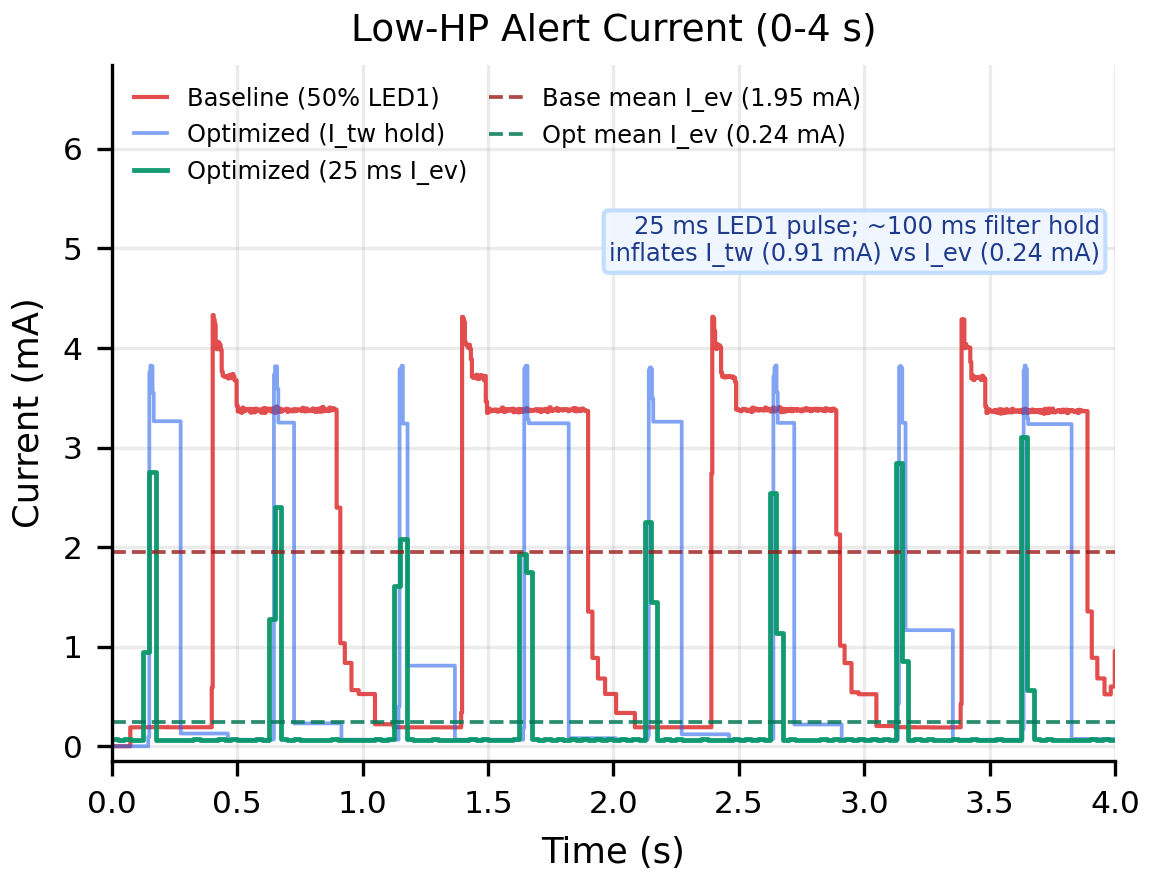
\includegraphics[width=\columnwidth]{figures/waveform_low_hp.png}
\caption{Low-HP Alert current (0--4~s): 25~ms $I_{\text{ev}}$ pulses ($243.4~\mu\text{A}$ mean) vs.\ Baseline 50\% \texttt{LED1} ($1,953.0~\mu\text{A}$) and $\sim$100~ms \texttt{EnergyTraceRunningAverageFilter} hold.}
\label{fig:wave_low_hp}
\end{figure}

\section{Datasheet Cross-Check \& Lifetime Projections}

Table~\ref{tab:datasheet} reconciles measured currents against TI's MSP430FR5994 datasheet~\cite{ti_ds}, LaunchPad User's Guide~\cite{ti_lp}, and Silicon Errata~\cite{ti_errata}. Measured \texttt{8~MHz LPM0} ($192.78~\mu\text{A}$) and \texttt{4~MHz LPM1} ($69.29~\mu\text{A}$ idle, $66.1$--$66.9~\mu\text{A}$ inter-tick) agree within $1.5\%$ and $1.7\%$--$6.6\%$ of typical $3.0\text{~V}$ specifications, with the small offset explained by $3.29\text{~V}$ supply, active 32.768~kHz LFXT, and eZ-FET \texttt{TXD}/\texttt{RXD} pull-ups.

\begin{table}[t]
\centering
\caption{MSP430FR5994 Datasheet (\texttt{SLASE54}), Schematic (\texttt{SLAU678C}), and Errata (\texttt{SLAZ681O}) Cross-Check}
\label{tab:datasheet}
\scriptsize
\setlength{\tabcolsep}{2.4pt}
\begin{tabular}{@{}llll@{}}
\toprule
Condition & Ref. & Spec Value & Measured ($I_{\text{ev}}$/$I_{p50}$) \\
\midrule
8~MHz \texttt{LPM0} & \texttt{SLASE54} & $190~\mu\text{A}$ typ & $192.8/189.9~\mu\text{A}$ ($+1.5\%$) \\
4~MHz \texttt{LPM1} & \texttt{SLASE54} & $65~\mu\text{A}$ typ & $69.3/69.2~\mu\text{A}$ ($66.1$--$66.9$ slp) \\
4~MHz TX/Act. & \texttt{SLASE54} & $\sim 590$--$680~\mu\text{A}$ & $\sim 610$--$650~\mu\text{A}$ TX plat. \\
8~MHz TX/Act. & \texttt{SLASE54} & $\sim 1.0$--$1.2\text{~mA}$ & $\sim 830$--$1,219~\mu\text{A}$ peaks \\
\texttt{LED1} (470~$\Omega$) & \texttt{SLAU678C} & $\approx 3.17\text{~mA}$ & $\sim 3.19\text{~mA}$ ($3.26$--$3.38$) \\
\texttt{PMM31/32/CS12} & \texttt{SLAZ681O} & \texttt{LPM1} exempt & 0 dropped B (8/8 pass) \\
\bottomrule
\end{tabular}
\end{table}

Using ideal energy budgets for a \textbf{CR2032} coin cell ($220\text{~mAh} \times 3.0\text{~V} = \mathbf{2,376\text{~J}}$, neglecting self-discharge/ESR cutoff) and the LaunchPad's on-board \textbf{\texttt{C1}} supercapacitor ($C_1=0.22\text{~F}$, $3.3\text{~V}\rightarrow 1.8\text{~V}$ usable span, $E_{C1} = \frac{1}{2} C_1 (V_{\max}^2 - V_{\min}^2) = \mathbf{0.8415\text{~J}}$ with \texttt{SVSHE=1} reset near $1.88\text{~V}$), Fig.~\ref{fig:lifetime} shows runtime increases from \textbf{43.37 to 120.63~days} (22.12 to 61.52~min on \texttt{C1}) in Idle, \textbf{34.10 to 60.53~days} in Active Play, \textbf{18.68 to 33.72--39.03~days} vs.\ active 8~MHz AI, and \textbf{4.28 to 34.35~days} (2.18 to 17.52~min on \texttt{C1}) in Low-HP Alert.

\begin{figure}[t]
\centering
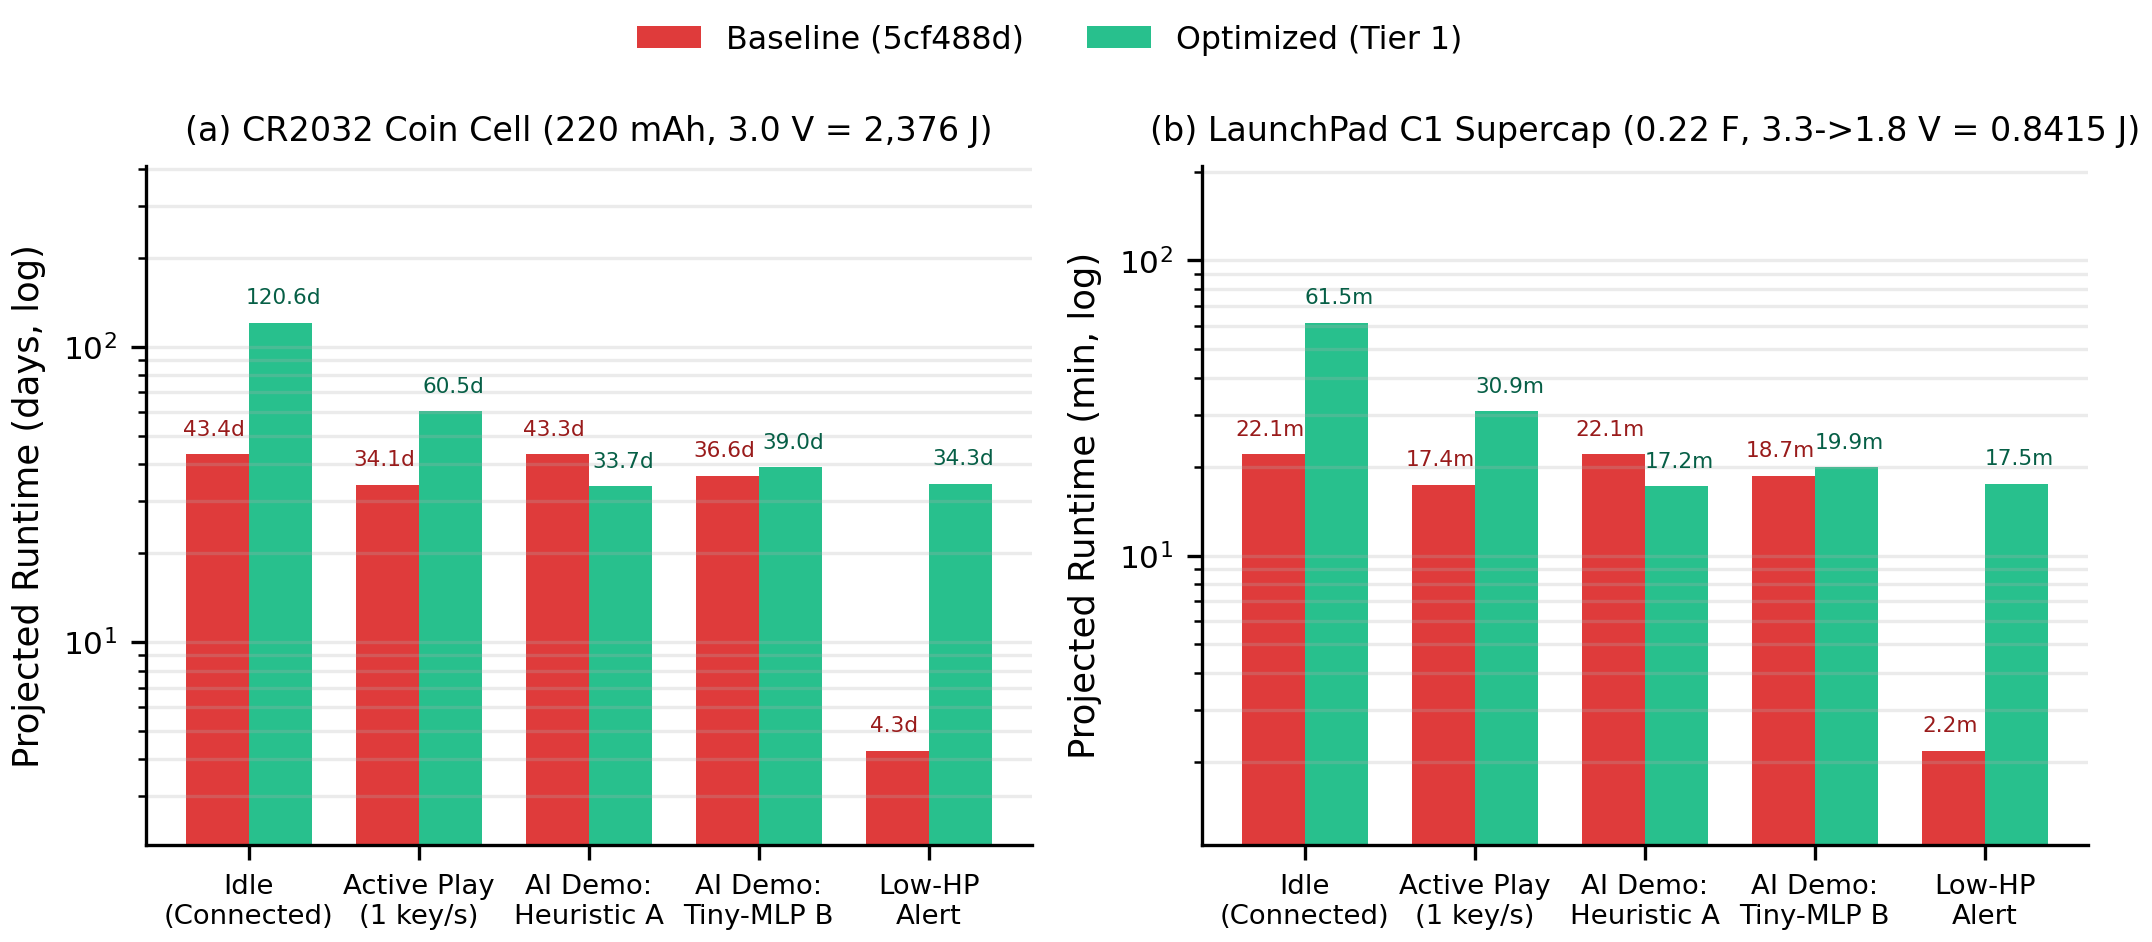
\includegraphics[width=\columnwidth]{figures/lifetime_projections.png}
\caption{Projected runtimes on (a) a 220~mAh CR2032 coin cell (2,376~J) and (b) the LaunchPad's 0.22~F supercapacitor \texttt{C1} (0.8415~J usable).}
\label{fig:lifetime}
\end{figure}

\section{Reproducibility \& Conclusion}
All artifacts are reproducible offline via \texttt{python tools/power\_plots.py} and \texttt{python tests/test\_e2e.py --require-final -v} (44/44 offline E2E checks passing). By diagnosing the \texttt{LPM3} $t_{\text{WAKE-UP}}$ / \texttt{PMM31} physical boundary and combining \texttt{PMM\_LPM1 @ 4~MHz}, 0~Hz dynamic \texttt{TIMER\_A1} gating, and 25~ms \texttt{LED1} pulses, \texttt{mspgame} achieves $1.78\times$--$8.02\times$ net power reductions with zero loss of interactive responsiveness.

\section*{AI Usage \& Assistance Disclaimer}
This work was directed, architected, and verified by the human author (\texttt{joaogpd}). AI coding and research assistants were used transparently as engineering aids to assist with auditing the low-level MSP430FR5994 peripheral drivers, developing the host-side benchmarking and EnergyTrace analysis scripts (\texttt{tools/power\_bench.py}, \texttt{tools/energytrace\_capture.py}, \texttt{tools/power\_plots.py}), running offline verification suites, and drafting documentation and manuscript text. All architectural decisions, physical MSP-EXP430FR5994 LaunchPad measurements, and reported metrics were verified under the human author's supervision, with every reported value derived strictly from raw EnergyTrace CSVs, TI documentation, and repository artifacts.

\begin{thebibliography}{5}
\bibitem{ti_ds} Texas Instruments, \emph{MSP430FR599x, MSP430FR596x Mixed-Signal Microcontrollers Datasheet (SLASE54)}, 2021.
\bibitem{ti_ug} Texas Instruments, \emph{MSP430FR58xx, MSP430FR59xx, and MSP430FR6xx Family User's Guide (SLAU367P)}, 2020.
\bibitem{ti_errata} Texas Instruments, \emph{MSP430FR5994 Device Erratasheet (SLAZ681O)}, 2021.
\bibitem{ti_lp} Texas Instruments, \emph{MSP430FR5994 LaunchPad Development Kit (MSP-EXP430FR5994) User's Guide (SLAU678C)}, 2019.
\bibitem{mspgame_ga} \texttt{joaogpd}, ``Evolving Zero-Float Q7 Autonomous Policies for a 16-Bit FRAM Microcontroller Roguelike,'' \emph{mspgame Project Technical Report} (\texttt{docs/ga/paper.tex}), 2026.
\end{thebibliography}

\end{document}
